\documentclass[UTF8]{ctexart}
\usepackage{subfigure}
\usepackage{caption}
\usepackage{amsmath,bm}
\usepackage{amssymb}
\usepackage{pifont}
\usepackage{geometry}
\usepackage{graphicx}
\usepackage{gensymb}
\usepackage{wrapfig}
\usepackage{titlesec}
\usepackage{float}
\usepackage{diagbox}
\usepackage{fancyhdr}
\usepackage{color}
\usepackage{bm}
\pagestyle{plain}
\geometry{a4paper,scale=0.8}
\CTEXsetup[format+={\raggedright}]{section} 
\title{固物2015期中A卷}
\author{Deschain}
\titlespacing*{\section}
{0pt}{0pt}{0pt}
\titlespacing*{\subsection}
{0pt}{0pt}{0pt}
\titlespacing*{\paragraph}
{0pt}{0pt}{0pt}
\titlespacing*{\subparagraph}
{0pt}{0pt}{0pt}
\titleformat*{\section}{\normalsize}
\begin{document}
\maketitle
\section*{\bfseries 1.填空题(每空1分,共34分)}
(1)布拉菲点阵中,能够完全平移覆盖的最小单元称为\uline{\makebox[3em]{}},每个单元含有
\uline{\makebox[2em]{}}个格点。\\
(2)Li、Na、K等碱金属的晶格属于\uline{\makebox[6em]{}}晶格,其中格点的面密度最大的晶面系的密勒指数为
\uline{\makebox[4em]{}}。设晶格常数为$a$,则该晶面系相邻晶面之间的面间距为\uline{\makebox[4em]{}}。\\
(3)晶体中面间距为$d$的一组晶面对应倒格子空间中的一个\uline{\makebox[3em]{}},这组晶面对应的倒格矢长
度为\uline{\makebox[3em]{}};若使用波长为$\lambda$的X射线对这一晶体进行衍射,则与这组平行晶面对应的一
级衍射峰的衍射角为\\
\uline{\makebox[9em]{}}。\\
(4)晶体中,空位与间隙原子都是典型的\uline{\makebox[2em]{}}缺陷。除此之外,晶体中的缺陷按其几何特征还
可以分为\uline{\makebox[2em]{}}缺陷和\uline{\makebox[2em]{}}缺陷。\\
(5)金刚石材料中C-C键结合的方式是典型的\uline{\makebox[6em]{}},其电离度为\uline{\makebox[2em]{}};
除了这种结合方式外,固体的结合方式还有\uline{\makebox[6em]{}},\uline{\makebox[6em]{}},
\uline{\makebox[9em]{}}。
(6)在索末菲自由电子模型中,对于一种二维材料,其总面积为$S$,则其对应的$k$空间的点阵密度为
\uline{\makebox[4em]{}},能量标度下自由电子的能态密度为\uline{\makebox[4em]{}}。\\
(7)布洛赫能带理论相比索末菲自由电子模型,主要是考虑了晶体中的\uline{\makebox[8em]{}}对电子运动的影响。
若电子简约波矢为$\vec{k}$,则电子的波函数具有性质:\uline{\makebox[15em]{}}。在近自由电子近似中,是以
\uline{\makebox[3em]{}}电子的本征值和本征函数作为零级解,将\uline{\makebox[10em]{}}看作微扰来求
解薛定谔方程的。\\
(8)布洛赫电子波函数的每个布里渊区内部的能级是\uline{\makebox[4em]{}}的,能级会在布里渊区的
\uline{\makebox[3em]{}}发生突变。在拓展布里渊区图景下,属于同一个布里渊区的能级构成一个
\uline{\makebox[3em]{}},两个能带之间不允许存在的能级宽度称为\uline{\makebox[3em]{}}。\\
(9)若电子占据了一个能带中所有的状态,则该能带\uline{\makebox[3em]{}}(能/不能)导电;没有任何电子占据
的能带\uline{\makebox[3em]{}}(能/不能)导电。\\
(10)能带顶部的电子有效质量为\uline{\makebox[2em]{}}(正/负),加速度为\uline{\makebox[2em]{}}(
正/负);能带底部的电子有效质量为\uline{\makebox[2em]{}}(正/负),加速度为\uline{\makebox[2em]{}}
(正/负)。
(11)在第一布里渊区中,电子的一个简约波矢对应了\uline{\makebox[3em]{}}(一个/多个)能量值。对于一维周期
势场中的布洛赫电子,其波函数为$\psi_k(x)=-isin(\frac{2x}{a}\pi)$,其中$a$为晶格常数,则电子的简约波矢为
\uline{\makebox[2em]{}}。\\
\section*{\bfseries 2.简答题(每题4分,共16分)}
(1)简述晶体中电子有效质量的物理意义。\\
(2)使用能带理论解释晶体中电子的能带和带隙是如何形成的。\\
(3)简述晶体、非晶体和准晶体之间的区别。\\
(4)用能带理论简述导体、绝缘体和半导体的区别。\\
\section*{\bfseries 3.(10分)如图所示,一个简单立方晶格的单胞,其晶格常数为$a$,K为AB中点。}
(1)写出OKC晶面的密勒指数;\\
(2)求OKC晶面的面间距。\\
\begin{figure}[H]
    \centering
    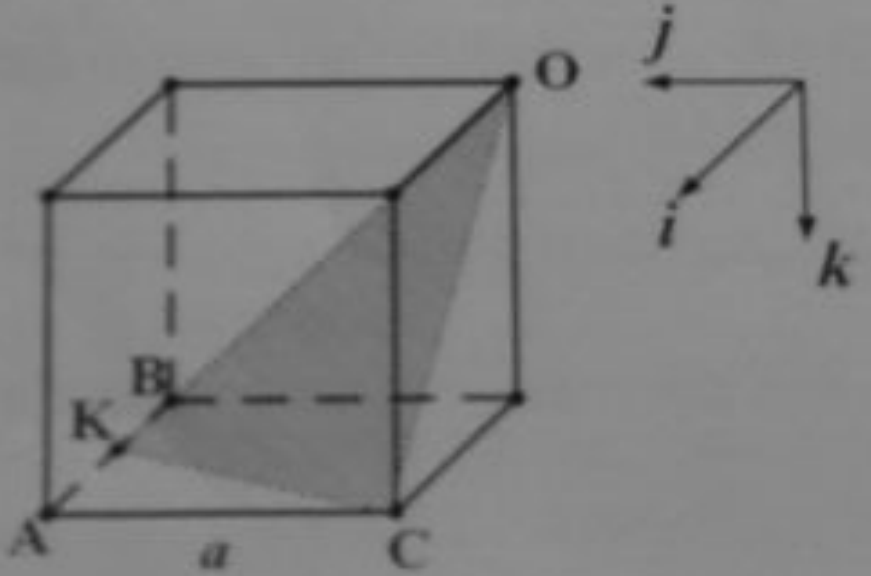
\includegraphics[width=6cm,height=4cm]{3.png}
\end{figure}
\section*{\bfseries 4.(10分)已知相距为$r$的两原子,相互作用势能可以表示为$U(r)=-\frac{\alpha}{r^m}+
\frac{\beta}{r_n}$,其中$\alpha,\beta,m,n$均为大于0的常数。}
(1)求出该系统的平衡位置和结合能。\\
(2)证明该系统可以处于稳定平衡态的条件是$n>m$。\\
\section*{\bfseries 5.(15分)设一维晶体的电子能带可以写成$E(k)=\frac{\hbar^2}{ma^2}(\frac{7}{8}-cos(ka)
+\frac{1}{8}cos(2ka))$,式中$a$为晶格常数,计算}
(1)能带的宽度;\\
(2)能带底部和能带顶部电子的有效质量。\\
(3)电子位于波矢$k$状态时的速度。\\
\section*{\bfseries 6.(15分)}
(1)假设金属钠单原子链的周期是$a$,单个原子感受到的周期性势场为
\begin{equation*}
    \begin{aligned}
        &V(x)=V_0cos(\frac{\pi x}{a})cos(\frac{3\pi x}{a}),V_0>0\\
    \end{aligned}
\end{equation*}
采用近自由电子近似,分别求出布里渊区边界$\frac{\pi}{a},\frac{2\pi}{a},\frac{3\pi}{a}$处的能隙,在下页图中画
出扩展布里渊区能带图,并判断其导电性。\\
(2)假设金属钠单原子链在低温下两两配对,晶格常数变为$2a$,此时若周期性势场的各级傅里叶展开系数均不为0,在下页
图中大致画出此时的扩展布里渊区能带结构示意图(至少画出三个布里渊区)。在不考虑能带交叠的情况下,此时系统导电性如
何?














\newpage
\section*{\bfseries 1.填空题}
(1)\ding{172}原胞\makebox[2em]{}
\ding{173}1\\
(2)\ding{172}体心立方\makebox[2em]{}
\ding{173}(100)或(101)或(011)\makebox[2em]{}
\ding{174}$\frac{\sqrt2}{2}a$\\
(3)\ding{172}点/格点/格矢\makebox[2em]{}
\ding{173}$\frac{2\pi}{d}$\makebox[2em]{}
\ding{174}$2arcsin(\frac{\lambda}{2d})$\\
(4)\ding{172}点\makebox[2em]{}
\ding{173}线\makebox[2em]{}
\ding{174}面\\
(5)\ding{172}共价键(共价结合)\makebox[2em]{}
\ding{173}0\makebox[2em]{}
\ding{174}离子键(离子结合)\makebox[2em]{}
\ding{175}金属键(金属性结合)\makebox[2em]{}
\ding{176}范德瓦耳斯力(范德瓦尔斯结合)\\
(6)\ding{172}$\frac{S}{4\pi^2}$\makebox[2em]{}
\ding{173}$\frac{mS}{\pi\hbar^2}$\\
(7)\ding{172}周期性势场\makebox[2em]{}
\ding{173}$\psi(\vec{r}+\vec{R_n})=e^{i\vec{k}\cdot\vec{R_n}}\cdot\psi(\vec{r})$\makebox[2em]{}
\ding{174}自由\makebox[2em]{}
\ding{175}周期性势场/周期性势场起伏/$\Delta V=V-V_0$\\
(8)\ding{172}准连续/分立\makebox[2em]{}
\ding{173}边界\makebox[2em]{}
\ding{174}能带\makebox[2em]{}
\ding{175}带隙/禁带\\
(9)\ding{172}不能\makebox[2em]{}
\ding{173}不能\\
(10)\ding{172}负\makebox[2em]{}
\ding{173}负\makebox[2em]{}
\ding{174}正\makebox[2em]{}
\ding{175}正\makebox[2em]{}
(11)\ding{172}多个\makebox[2em]{}
\ding{173}0\\
\section*{\bfseries 2.简答题答案}
(1)晶体中的电子(或空穴)除了受到外场作用外,还要受到晶体中原子的周期性势场和其他电子的平均势场的作用。在讨论电子
受外场力作用下运动时,有效质量即是把内场力等价为电子的一部分质量后得到的结果。有效质量的表达式为
$\frac{1}{{m_\alpha}^{*}}=\frac{1}{\hbar^2}\cdot\frac{\partial^2E}{{\partial k_\alpha}^2}$\\
(2)\ding{172}能带:由于周期性边界条件,$\bm{k}$的取值是分立的。当原子数趋于无穷时,能级变得准连续,形成能带。\\
\ding{173}带隙:在近自由电子近似模型中,晶格的周期性势场被看做微扰。在布里渊区的边界,波函数是简并的。根据简并微扰
模型,会发生能级劈裂,也就形成了带隙。\\
(3)\ding{172}晶体:内部原子排布具有周期性。\\
\ding{173}非晶体:内部原子排布没有周期性。\\
\ding{174}准晶体:内部原子排布具有旋转对称性,没有平移对称性。(或具有长程取向序,无长程平移序)\\
(4)\ding{172}导体:价带完全填充,导带部分填充。\\
\ding{173}绝缘体:价带完全填充,导带全空,并且带隙较大,不易发生跃迁。\\
\ding{174}半导体:绝对零度时,价带、导带的填充情况与绝缘体相同。但是带隙较小,室温下,一部分电子可以从价带上被热激发
到导带上。导带和价带都变成部分填充,可以导电。\\
\section*{\bfseries 3.解答}
(1)$(2,1,\overline{2})$\\
(2)$\frac{a}{3}$\\
\section*{\bfseries 4.解答}
(1)设平衡位置为$r_0$,结合能为$W$。
\begin{equation*}
    \begin{aligned}
        & \frac{dU(r)}{dr}=\frac{m\alpha}{r^{m+1}}-\frac{n\beta}{r^{n+1}}\\
        & \frac{dU(r_0)}{dr}=0,r_0=(\frac{n\beta}{m\alpha})^{\frac{1}{m-n}}\\
        & W=-U(r_0)=\alpha(\frac{m\alpha}{n\beta})^{\frac{m}{n-m}}-\beta(\frac{m\alpha}{n\beta})^{\frac{n}{n-m}}\\
    \end{aligned}
\end{equation*}
(2)
\begin{equation*}
    \begin{aligned}
        & \frac{d^2U}{dr^2}\lvert_{r=r_0}>0 \iff n>m
    \end{aligned}
\end{equation*}
\section*{\bfseries 5.解答}
(1)
\begin{equation*}
    \begin{aligned}
        & \Delta E=E(\frac{\pi}{a})-E(0)=\frac{2\hbar^2}{ma^2}\\
    \end{aligned}
\end{equation*}
(2)
\begin{equation*}
    \begin{aligned}
        & m^*=\frac{\hbar^2}{\frac{\partial^2E}{\partial k^2}}=\frac{m}{cos(ka)-\frac{1}{2}cos(2ka)}\\
        & m^*(0)=2m, m^*(\frac{\pi}{a})=-\frac{2}{3}m\\
    \end{aligned}
\end{equation*}
(3)
\begin{equation*}
    \begin{aligned}
        & v=\frac{1}{\hbar}\frac{\partial E}{\partial k}=\frac{\hbar}{ma}(sin(ka)-\frac{1}{4}sin(2ka))\\
    \end{aligned}
\end{equation*}
\section*{\bfseries 6.解答}
(1)
\begin{equation*}
    \begin{aligned}
        & V(x)=\frac{V_0}{4}(e^{i\frac{4\pi}{a}x}+e^{i\frac{2\pi}{a}x}+e^{-i\frac{2\pi}{a}x}
        +e^{-i\frac{4\pi}{a}x})\\
        & V_{\pm1}=V_{\pm2}=\frac{V_0}{4}\\
    \end{aligned}
\end{equation*}
常温下,第一能带部分填充,导电性良好。\\
\begin{figure}[H]
    \centering
    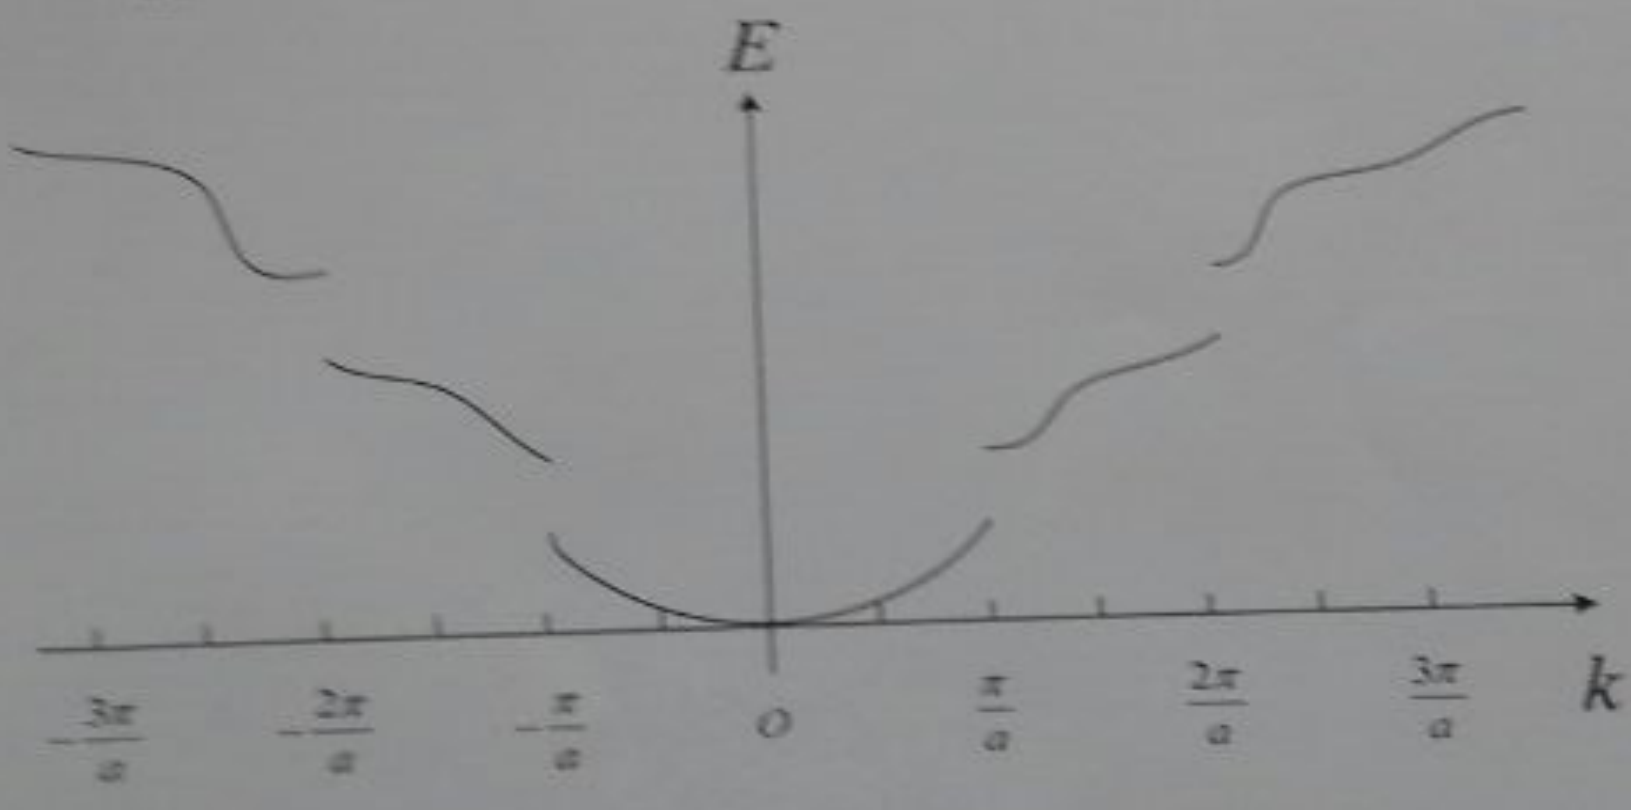
\includegraphics[width=6cm,height=4cm]{6_1.png}
\end{figure}
(2)晶格常数改变,造成倒格矢的大小改变,一个能带内能够容纳的状态数减半,因此原本半满的能带变成了满带,不导电。\\
常温下,第一能带部分填充,导电性良好。\\
\begin{figure}[H]
    \centering
    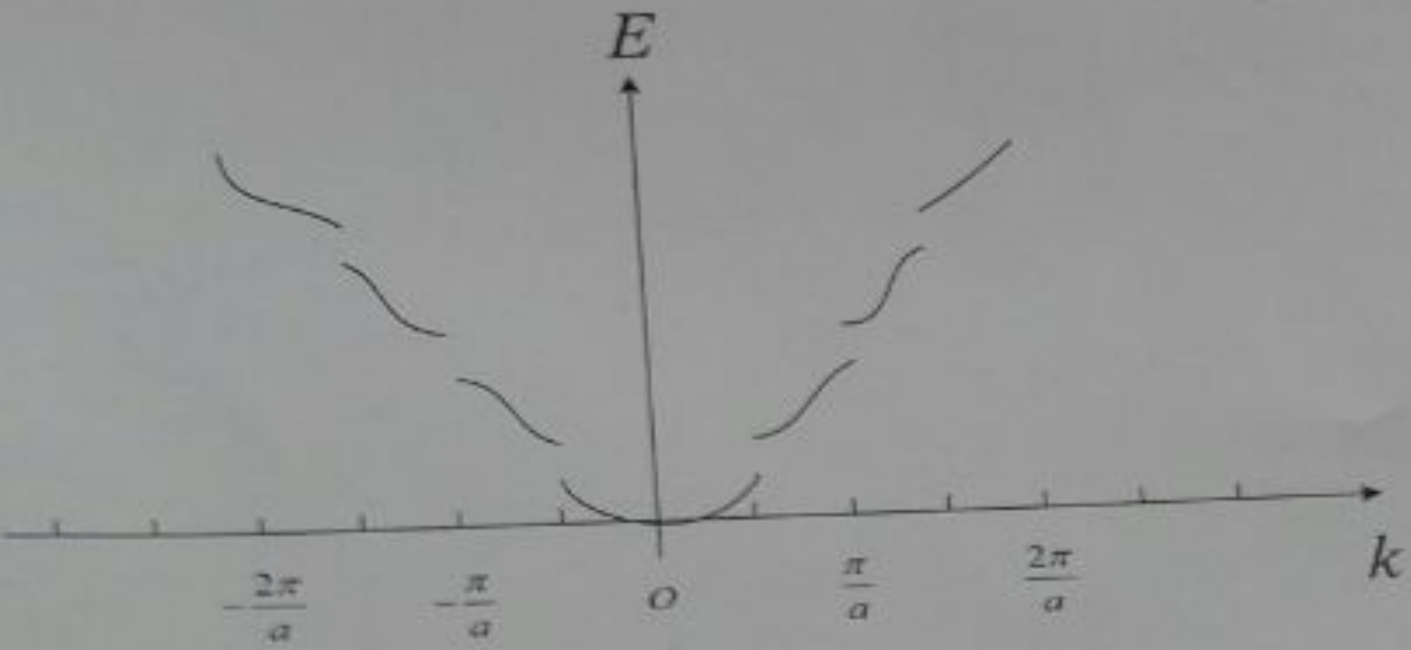
\includegraphics[width=6cm,height=4cm]{6_2.png}
\end{figure}
\end{document}